\documentclass{beamer}\usepackage[]{graphicx}\usepackage[]{color}
% maxwidth is the original width if it is less than linewidth
% otherwise use linewidth (to make sure the graphics do not exceed the margin)
\makeatletter
\def\maxwidth{ %
  \ifdim\Gin@nat@width>\linewidth
    \linewidth
  \else
    \Gin@nat@width
  \fi
}
\makeatother

\definecolor{fgcolor}{rgb}{0.345, 0.345, 0.345}
\newcommand{\hlnum}[1]{\textcolor[rgb]{0.686,0.059,0.569}{#1}}%
\newcommand{\hlstr}[1]{\textcolor[rgb]{0.192,0.494,0.8}{#1}}%
\newcommand{\hlcom}[1]{\textcolor[rgb]{0.678,0.584,0.686}{\textit{#1}}}%
\newcommand{\hlopt}[1]{\textcolor[rgb]{0,0,0}{#1}}%
\newcommand{\hlstd}[1]{\textcolor[rgb]{0.345,0.345,0.345}{#1}}%
\newcommand{\hlkwa}[1]{\textcolor[rgb]{0.161,0.373,0.58}{\textbf{#1}}}%
\newcommand{\hlkwb}[1]{\textcolor[rgb]{0.69,0.353,0.396}{#1}}%
\newcommand{\hlkwc}[1]{\textcolor[rgb]{0.333,0.667,0.333}{#1}}%
\newcommand{\hlkwd}[1]{\textcolor[rgb]{0.737,0.353,0.396}{\textbf{#1}}}%
\let\hlipl\hlkwb

\usepackage{framed}
\makeatletter
\newenvironment{kframe}{%
 \def\at@end@of@kframe{}%
 \ifinner\ifhmode%
  \def\at@end@of@kframe{\end{minipage}}%
  \begin{minipage}{\columnwidth}%
 \fi\fi%
 \def\FrameCommand##1{\hskip\@totalleftmargin \hskip-\fboxsep
 \colorbox{shadecolor}{##1}\hskip-\fboxsep
     % There is no \\@totalrightmargin, so:
     \hskip-\linewidth \hskip-\@totalleftmargin \hskip\columnwidth}%
 \MakeFramed {\advance\hsize-\width
   \@totalleftmargin\z@ \linewidth\hsize
   \@setminipage}}%
 {\par\unskip\endMakeFramed%
 \at@end@of@kframe}
\makeatother

\definecolor{shadecolor}{rgb}{.97, .97, .97}
\definecolor{messagecolor}{rgb}{0, 0, 0}
\definecolor{warningcolor}{rgb}{1, 0, 1}
\definecolor{errorcolor}{rgb}{1, 0, 0}
\newenvironment{knitrout}{}{} % an empty environment to be redefined in TeX

\usepackage{alltt}
\usepackage{../371g-slides}
\title{Probability 1}
\subtitle{Lecture 2}
\author{STA 371G}
\IfFileExists{upquote.sty}{\usepackage{upquote}}{}
\begin{document}



  \frame{\maketitle}

  % Show outline at beginning of each section
  \AtBeginSection[]{
    \begin{frame}<beamer>
      \tableofcontents[currentsection]
    \end{frame}
  }

  %%%%%%% Slides start here %%%%%%%

  \begin{darkframes}
    \section{Announcements and logistics}

    \begin{frame}{Announcements}
      \begin{itemize}
        \item You can find lecture slides, data, etc on Canvas
        \item Practice quiz tomorrow night at 6:30 PM (15 minutes, doesn't count towards your grade!)
      \end{itemize}
    \end{frame}

    \begin{frame}{}
      \fullpagepicture{convergent1.png}
    \end{frame}
    \begin{frame}{}
      \fullpagepicture{convergent2.png}
    \end{frame}
    \begin{frame}{}
      \fullpagepicture{convergent3.png}
    \end{frame}
   
    \section{Probability rules}

    \begin{frame}{Probability rules}
      \begin{enumerate}
        \item The chance of an event happening is between 0\% and 100\%, i.e. $0 \leq P(E) \leq 1$ for any event $E$.
        \item The probabilities for all possible outcomes put together add up to 1.
        \item The probability that something doesn’t happen is 100\% minus the probability that it does happen, i.e. $P(E^c) = 1-P(E)$.
      \end{enumerate}
    \end{frame}

    \begin{frame}{Disjoint events}
      \begin{definition}
        Two events $A$ and $B$ are \alert{disjoint} if they never both occur, i.e., if $P(\text{$A$ and $B$}) = 0$.        
      \end{definition}

      \pause

      If we consider two UT students selected at random,
      \begin{itemize}
        \item ``Has as 3.0 GPA'' and ``Has a 4.0 GPA'' are disjoint
        \item ``Has a major in McCombs'' and ``Has a major in CNS'' are not disjoint (you can do both!)
      \end{itemize}
    \end{frame}


    \begin{frame}{}
      \begin{center}
        Let's say we pick a \emph{Jersey Shore: Family Vacation} cast member at random.
      \end{center}
      

      
\includegraphics[width=\textwidth]{jersey-shore}
    \end{frame}

    \begin{frame}{}
      \begin{center}
        \begin{tabular}{cccc}
          
\includegraphics[width=0.8in]{mike} & 
          
\includegraphics[width=0.8in]{ronnie} &
          
\includegraphics[width=0.8in]{vinny} &
          
\includegraphics[width=0.8in]{pauly} \\
          Mike & Ronnie & Vinny & Pauly \\
          
\includegraphics[width=0.8in]{jwoww} &
          
\includegraphics[width=0.8in]{snooki} &
          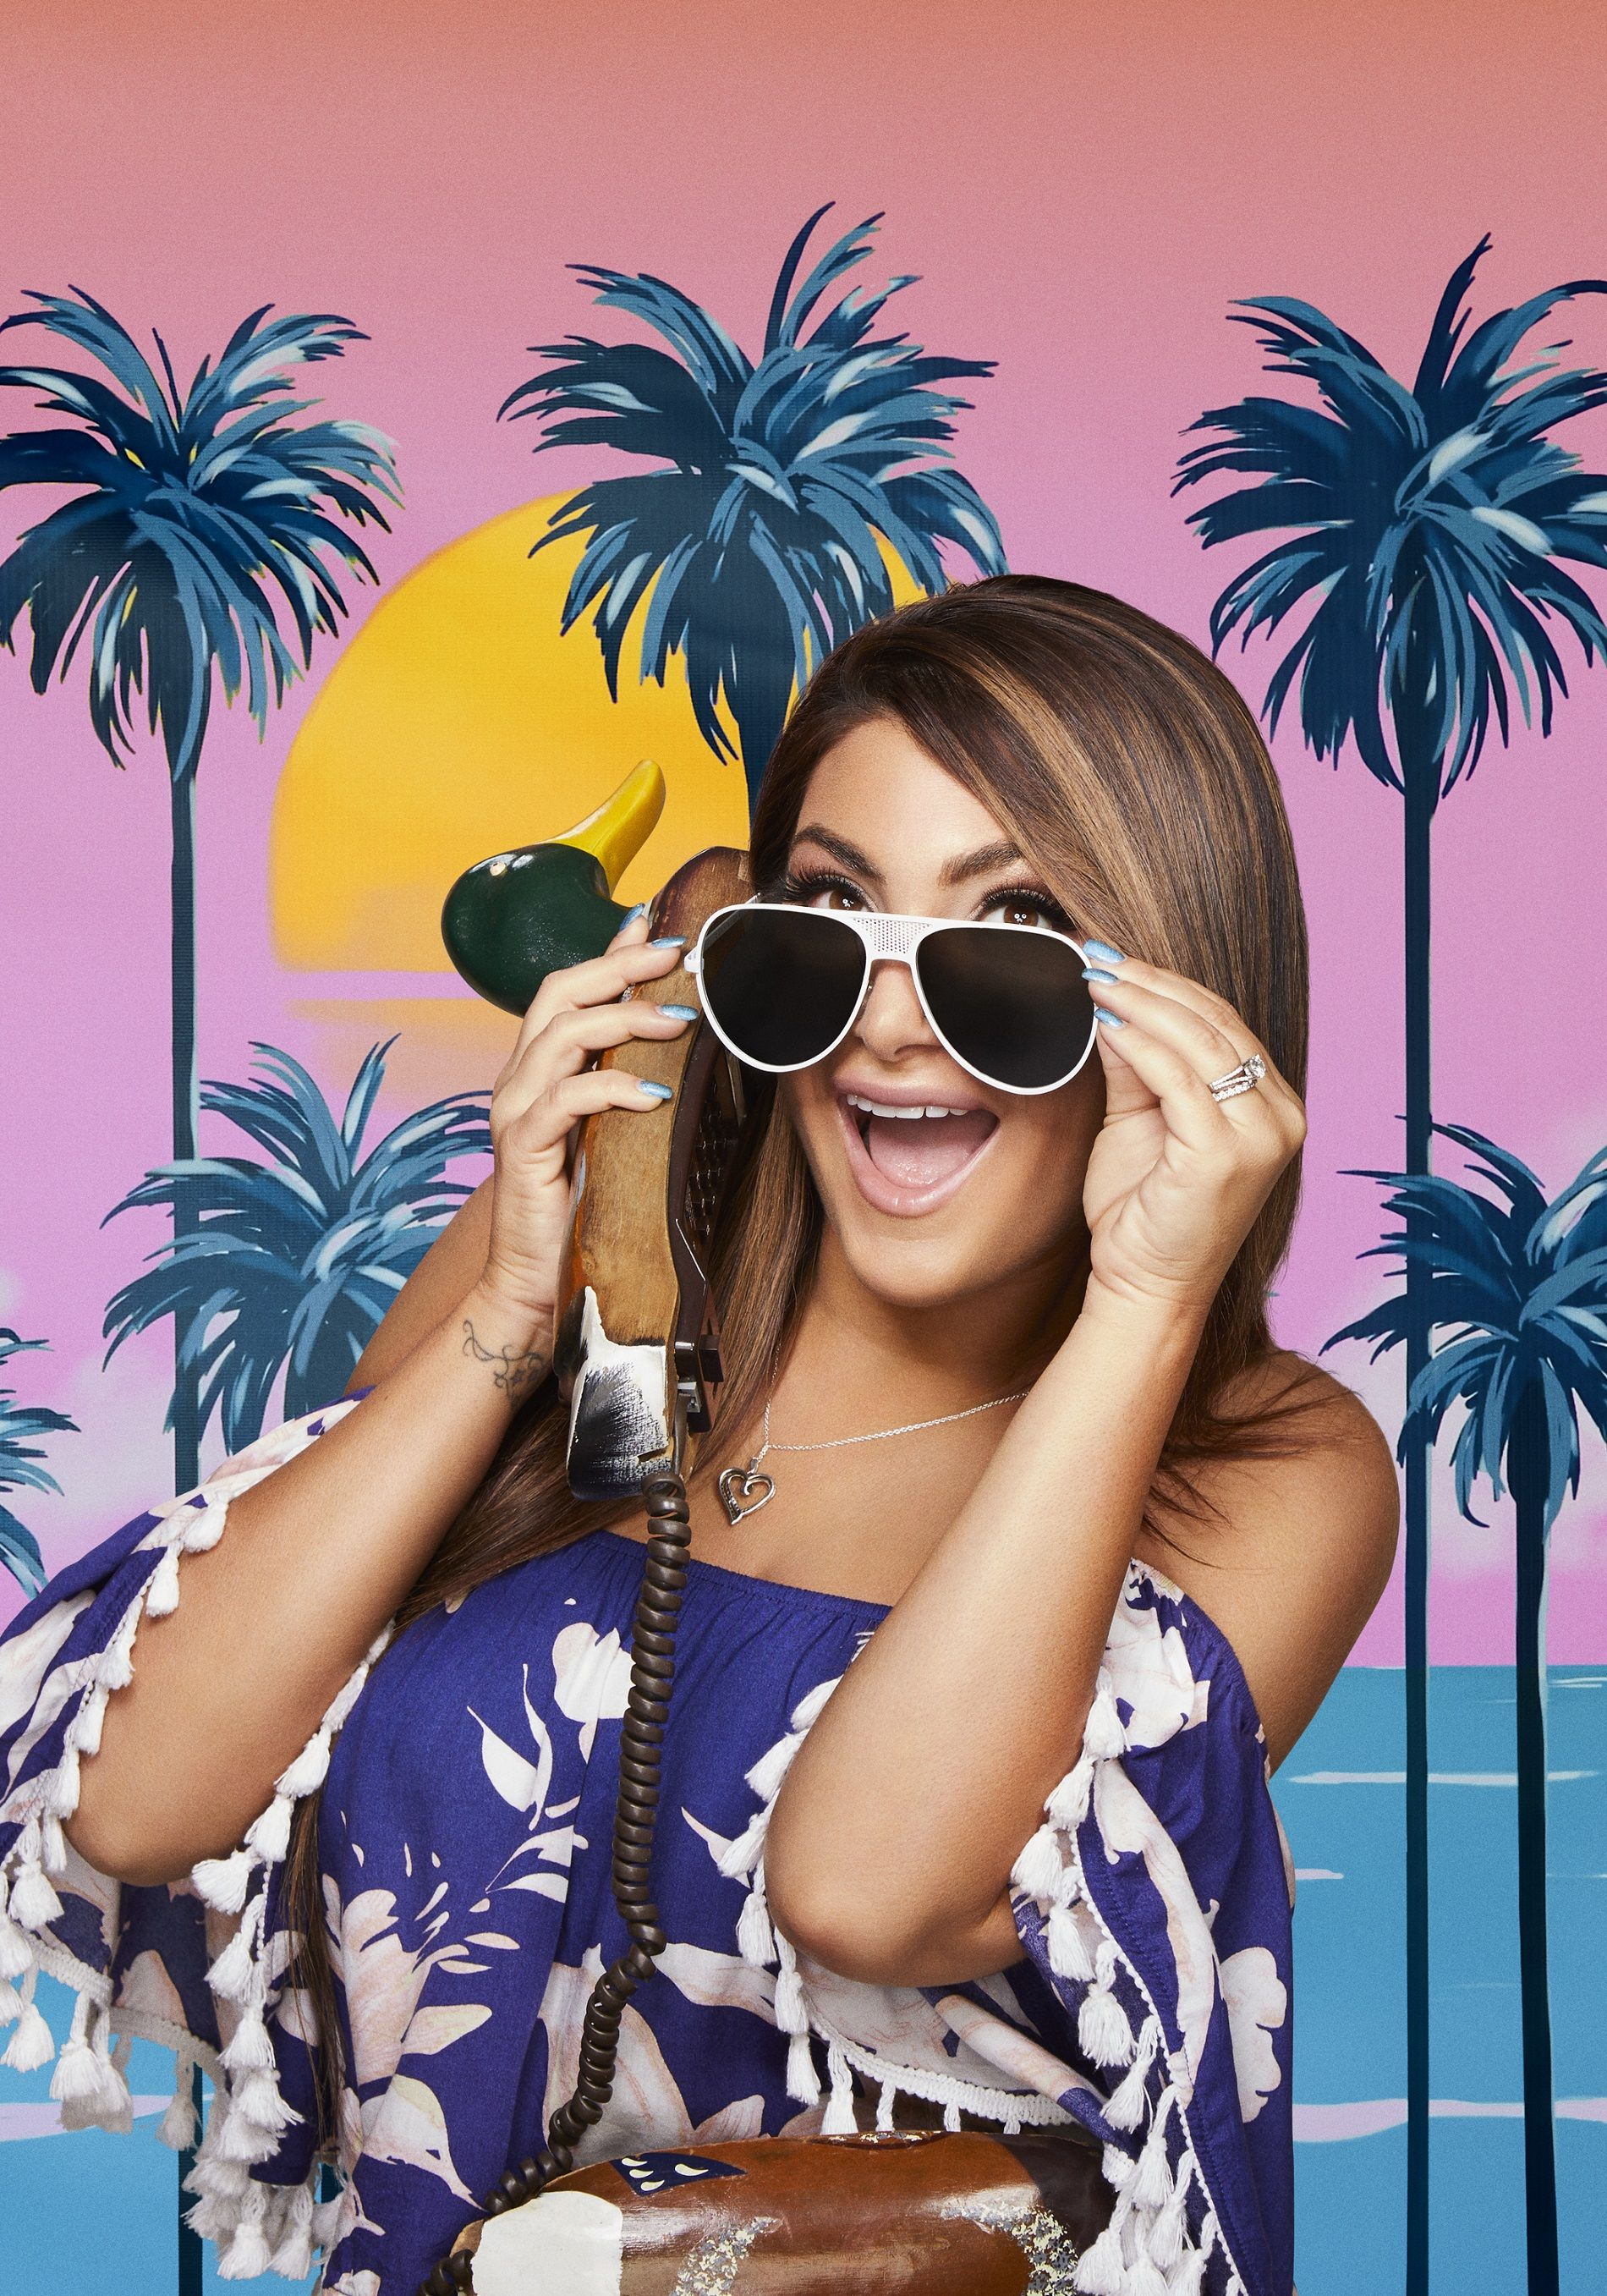
\includegraphics[width=0.8in]{deena} &
          
\includegraphics[width=0.8in]{angelina} \\
          J-Woww & Snooki & Deena & Angelina \\
        \end{tabular}
      \end{center}
    \end{frame}

    \begin{frame}{Probability rules}
      \begin{enumerate}
        \item The chance of an event happening is between 0\% and 100\%, i.e. $0 \leq P(E) \leq 1$ for any event $E$.
        \item The probabilities for all possible outcomes put together add up to 1.
        \item The probability that something doesn’t happen is 100\% minus the probability that it does happen, i.e. $P(E^c) = 1-P(E)$.
        \item If $A$ and $B$ are disjoint, $P(\text{$A$ or $B$}) = P(A)+P(B)$.
      \end{enumerate}
    \end{frame}

    \begin{frame}{What if the events are not disjoint?}
      \begin{center}
        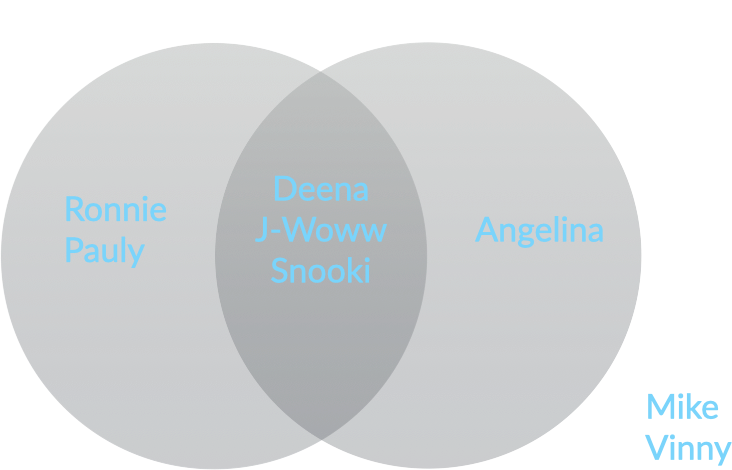
\includegraphics[width=3in]{venn}
      \end{center}
      
      \[
        P(C) = \frac 5 8 \qquad P(F) = \frac 4 8 
        \qquad P(\text{$C$ or $F$}) = \frac 6 8 \neq P(C) + P(F)
      \]
    \end{frame}

    \begin{frame}{What if the events are not disjoint?}
      \begin{center}
        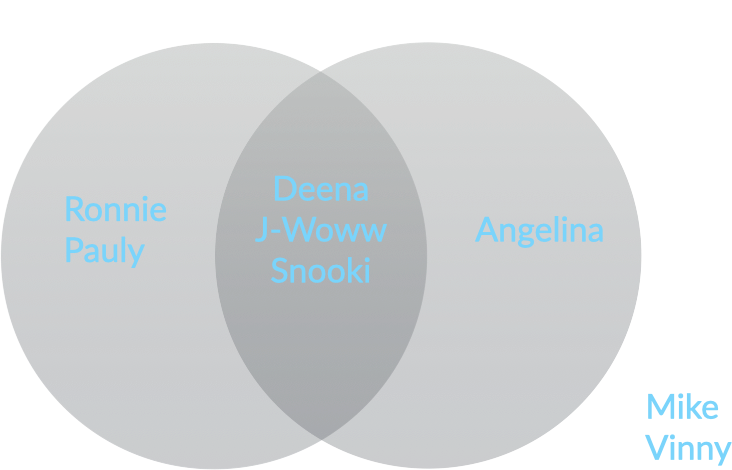
\includegraphics[width=3in]{venn}
      \end{center}
      
      We are double-counting Deena, J-Woww, and Snooki! 
      \[
        \qquad P(\text{$C$ or $F$}) = P(C) + P(F) - P(\text{$C$ and $F$}) = \frac 5 8 + \frac 4 8 - \frac 3 8 = \frac 6 8
      \]
    \end{frame}

    \begin{frame}{Probability rules}
      \begin{enumerate}
        \item The chance of an event happening is between 0\% and 100\%, i.e. $0 \leq P(E) \leq 1$ for any event $E$.
        \item The probabilities for all possible outcomes put together add up to 1.
        \item The probability that something doesn’t happen is 100\% minus the probability that it does happen, i.e. $P(E^c) = 1-P(E)$.
        \item $P(\text{$A$ or $B$}) = P(A)+P(B) - P(\text{$A$ and $B$})$.
      \end{enumerate}
    \end{frame}

    \begin{frame}{Independent events}
      \begin{definition}
        Two events $A$ and $B$ are \alert{independent} if knowing that one event happened tells you nothing about whether the other happened.        
      \end{definition}

      \pause

      If we consider two UT students selected at random,
      \begin{itemize}
        \item ``Has blue eyes'' and ``Has a 4.0 GPA'' are independent
        \item ``Got a 1600 on their SAT'' and ``Has a 4.0 GPA'' are not independent
      \end{itemize}
    \end{frame}


    \begin{frame}{Probability rules}
      \begin{enumerate}
        \item The chance of an event happening is between 0\% and 100\%, i.e. $0 \leq P(E) \leq 1$ for any event $E$.
        \item The probabilities for all possible outcomes put together add up to 1.
        \item The probability that something doesn’t happen is 100\% minus the probability that it does happen, i.e. $P(E^c) = 1-P(E)$.
        \item $P(\text{$A$ or $B$}) = P(A)+P(B) - P(\text{$A$ and $B$})$.
        \item If $A$ and $B$ are independent, $P(\text{$A$ and $B$}) = P(A)P(B)$.
      \end{enumerate}
    \end{frame}

    \begin{frame}{What if the events are not independent?}
      \begin{center}
        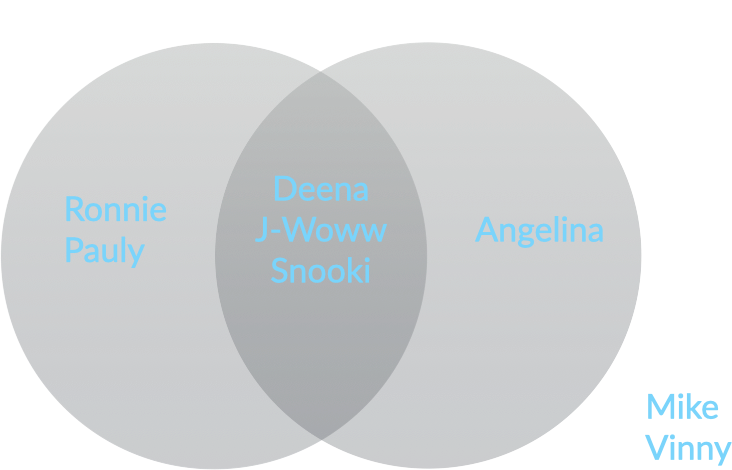
\includegraphics[width=3in]{venn}
      \end{center}
      
      We are double-counting Deena, J-Woww, and Snooki! 
      \[
        P(C) = \frac 5 8 \qquad P(F) = \frac 4 8 
        \qquad P(\text{$C$ and $F$}) = \frac 3 8 \neq P(C) P(F)
      \]
    \end{frame}

    \section{Getting our hands dirty with R}

    \begin{frame}{A quick overview of R}
      \begin{itemize}
        \item Data window, console window, environment window, plot/help window
        \item Using R as a calculator
        \item Using the console window
        \item Creating R scripts (why and how)
        \item Adding comments to scripts
        \item Importing data from a spreadsheet
        \item Loading RData files
      \end{itemize}
    \end{frame}

    \begin{frame}[fragile]{Summarizing categorical data}
      Use the \verb|table| function to create a contingency (frequency) table for categorical data:
\begin{knitrout}
\definecolor{shadecolor}{rgb}{0.969, 0.969, 0.969}\color{fgcolor}\begin{kframe}
\begin{alltt}
\hlkwd{table}\hlstd{(titanic}\hlopt{$}\hlstd{Sex, titanic}\hlopt{$}\hlstd{Survived)}
\end{alltt}
\begin{verbatim}
        
          No Yes
  female  71 217
  male   372  96
\end{verbatim}
\end{kframe}
\end{knitrout}
    \end{frame}

    \begin{frame}[fragile]
      Use the \verb|addmargins| function to add ``margins'' (the row, column, and overall totals):
\begin{knitrout}
\definecolor{shadecolor}{rgb}{0.969, 0.969, 0.969}\color{fgcolor}\begin{kframe}
\begin{alltt}
\hlkwd{addmargins}\hlstd{(}\hlkwd{table}\hlstd{(titanic}\hlopt{$}\hlstd{Sex, titanic}\hlopt{$}\hlstd{Survived))}
\end{alltt}
\begin{verbatim}
        
          No Yes Sum
  female  71 217 288
  male   372  96 468
  Sum    443 313 756
\end{verbatim}
\end{kframe}
\end{knitrout}
    \end{frame}

    \begin{frame}[fragile]
      Apply \verb|prop.table| to a table to tally up percentages by rows or columns:
\begin{knitrout}
\definecolor{shadecolor}{rgb}{0.969, 0.969, 0.969}\color{fgcolor}\begin{kframe}
\begin{alltt}
\hlcom{# By rows}
\hlkwd{prop.table}\hlstd{(}\hlkwd{table}\hlstd{(titanic}\hlopt{$}\hlstd{Sex, titanic}\hlopt{$}\hlstd{Survived),} \hlnum{1}\hlstd{)}
\end{alltt}
\begin{verbatim}
        
                No       Yes
  female 0.2465278 0.7534722
  male   0.7948718 0.2051282
\end{verbatim}
\begin{alltt}
\hlcom{# By columns}
\hlkwd{prop.table}\hlstd{(}\hlkwd{table}\hlstd{(titanic}\hlopt{$}\hlstd{Sex, titanic}\hlopt{$}\hlstd{Survived),} \hlnum{2}\hlstd{)}
\end{alltt}
\begin{verbatim}
        
                No       Yes
  female 0.1602709 0.6932907
  male   0.8397291 0.3067093
\end{verbatim}
\end{kframe}
\end{knitrout}
    \end{frame}

    \begin{frame}{Getting more help with R}
      Additional resources for learning R are available on Canvas (see also the STA 309 R help pages if you are new to R).
    \end{frame}
  \end{darkframes}
\end{document}
